% \documentclass[10pt, oneside, english]{article}   	
\documentclass[10pt, oneside]{article}
\usepackage{geometry}                		
\geometry{a4paper}                   		
% \usepackage[english, es-noindentfirst]{babel}
% \selectlanguage{english}
\usepackage[utf8]{inputenc}               		
\usepackage{graphicx}			
\usepackage{amssymb}
\usepackage{authblk}
\usepackage{multicol}
\usepackage{rotating}


\title{Word embeddings for predicting political affiliation based on Twitter data}

\author[]{Ibrahim Abdelaziz}
\author[]{Oliver Berg}
\author[]{Angjela Davitkova}
\author[]{Venkatesh Iyer}
\author[]{Shriram Selvakumar}
\author[]{Kumar Shridhar}
\author[]{Saurabh Varshneya}
\affil[1]{Technische Universität Kaiserslautern}

\date{\today}


\begin{document}
\maketitle
\begin{multicols}{2}


\section{Introduction}

The modern world of social media knows a plethora of means to communicate ones personal opinion and political alignment. With the platform \textit{Twitter}, figures of political interest are expressing their standpoints in small-sized 144 character texts (recently updated to 280 characters), which contain a comprised message specific to the general public. This yields great potential for automated analysis of party affiliations to classify political persons of interest within the overall political spectrum \cite{Biessmann2017}.

Hence, we propose a structured approach of building a deep learning based classification model that utilizes state-of-the-art \textbf{word embeddings} \cite{Pelevinala2016} to perform \textbf{qualitative analysis} on a constructed \textbf{social media data set}. Our approach will be helpful in analyzing possible early intuitions and dedicated insights within the German political spectrum.

This is to be seen in context of latest \textbf{advances in research}.


\section{Related Work}

Political motives were shown to be consistently predictable with an accuracy better than chance \cite{Biessmann2017}.

Many existing papers either propose tackling the classification problem of political bias using techniques such as Support Vector Machine (SVM) or Singular Value Decomposition (SVD) \cite{Misra2016}, or they focus on comparison of different classifiers to not restrict themselves to a single well-developed approach \cite{Bhanda2009}. These approaches mainly consider the political affiliation in America, where the political orientation is mostly binary with two parties - republicans and democrats - covering most of the political spectrum.
Overall, sentiment classification is mostly covered using recurrent- or convolutional neural networks \cite{Kim2014}.

In connection to the given focus of working on Twitter data, \cite{Cohen2013} introduces objections to some of the pre-existing approaches. With standard classifiers for inferring political orientation having greatly lower accuracy compared to what was initially report, it is stated that the classifiers cannot be used for classifying users outside the training data. Thus the contradictory arguments hold true.


\section{Proposed Methodology}

As our approach aims to analyze text messages of political figures concerning party affiliation, we leverage \textit{word embeddings} to represent words in context. We shall initially restrict ourselves to a pre-trained model as the number of political parties as classes is not very high. A person's political affiliation will be calculated as a combined analysis of all of his Twitter messages.

Subsequently, a neural network architecture then classifies the Twitter profile, consisting of a collection of this person's tweets, concerning party affiliation. It will learn to represent a political figure's affiliation through their expression in short message texts.

\subsection{Data Sets and Feature Extraction} 

The main portion of data collected will be Twitter data. In order to include all of the relevant politicians from all considered parties, their Twitter accounts with their corresponding messages will be collected, where the data is offered as open source data.
Each politicians own party is kept as his ground truth class label.

In order to train models on text, the data needs to be converted into numerical values, more specifically vectors, under specific similarity metrics. One way this can be achieved is to create a word embedding for each of the words from the tweets using \textit{Word2Vec} \cite{DBLP:journals/corr/abs-1301-3781}. While constructing word embeddings, appropriate dimensionality reduction can be applied.

There are seven class labels as there are seven political parties considered, namely "CDU", "CSU", SPD", "FDP", "GRÜNE", "LINKE" and "AFD", ordered by age of introduction into German parliament, old to new. As such, a pre-trained word embeddings model should suffice to represent textual influence in regard to this relatively small number of classes.
Alternatively, a custom model may be trained on a Wikipedia data dump in German language, possibly in combination with more politically motivated data sources such as German parliament discussion data or party manifesto data. 

For each party, the same number of accounts and tweets per account will be used to later train the classification model.

Train-test-splits with ration 80-20 will be employed, where the collection of a single person's tweets will be counted as a single data record. It may not be humanly feasible to classify a person's party affiliation based on a single Twitter message, and as such this should also not be the classifier's primary objective.

To recap, we propose to accumulate twitter-data per political figure and treat this collection as singular data records. Each record is associated with a single class label, depicting his truly associated party. Records are represented in numerical format by applying word embedding techniques. 

\subsection{Classification}

While deciding upon the architecture, RNN(Recurrent Neural Network) looked like an intuitive solution as it is more similar to how humans think and process language: one word at a time and then forming sentence using those words. But we wanted to experiment things in terms of making the training process faster and less computational intensive, so we used a CNN model for our case as convolutions are a central part of computer graphics and implemented on a hardware level on GPUs which make them very fast for training.

Another point in favor of CNN is being very efficient in representations.  With a large vocabulary, computing anything more than 3-grams can quickly become expensive.  Convolutional Filters learn good representations automatically, without needing to represent the whole vocabulary and we can put a bigger filter size of 7 or more depending on the use cases as different filter sizes learn different representations. 

\subsubsection{Model Architecture}

Our model architecture is taken from [[]] which is used for sentiment analysis. The first layers embeds words into low-dimensional vectors. The next layer performs convolutions over the embedded word vectors using multiple filter sizes. For example, sliding over 3, 4 or 5 words at a time. Next, we max-pool the result of the constitutional layer into a long feature vector, add dropout regularization, and classify the result using a softmax layer.


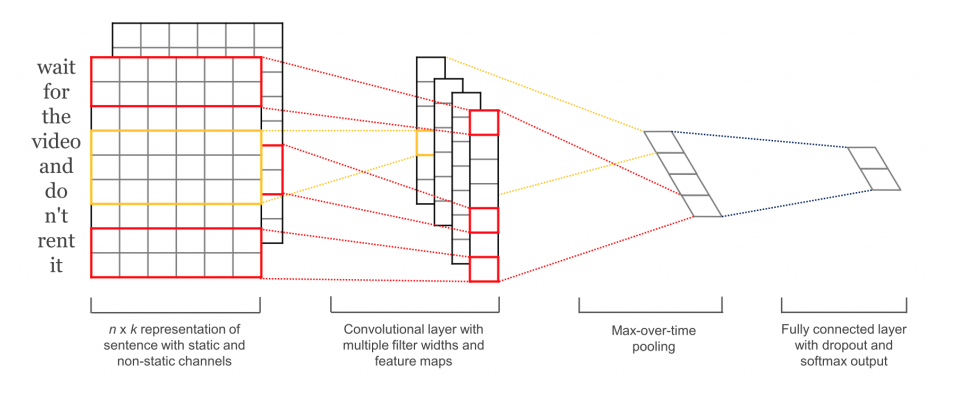
\includegraphics[width=0.5\textwidth]{images/cnn_architecture1.png}
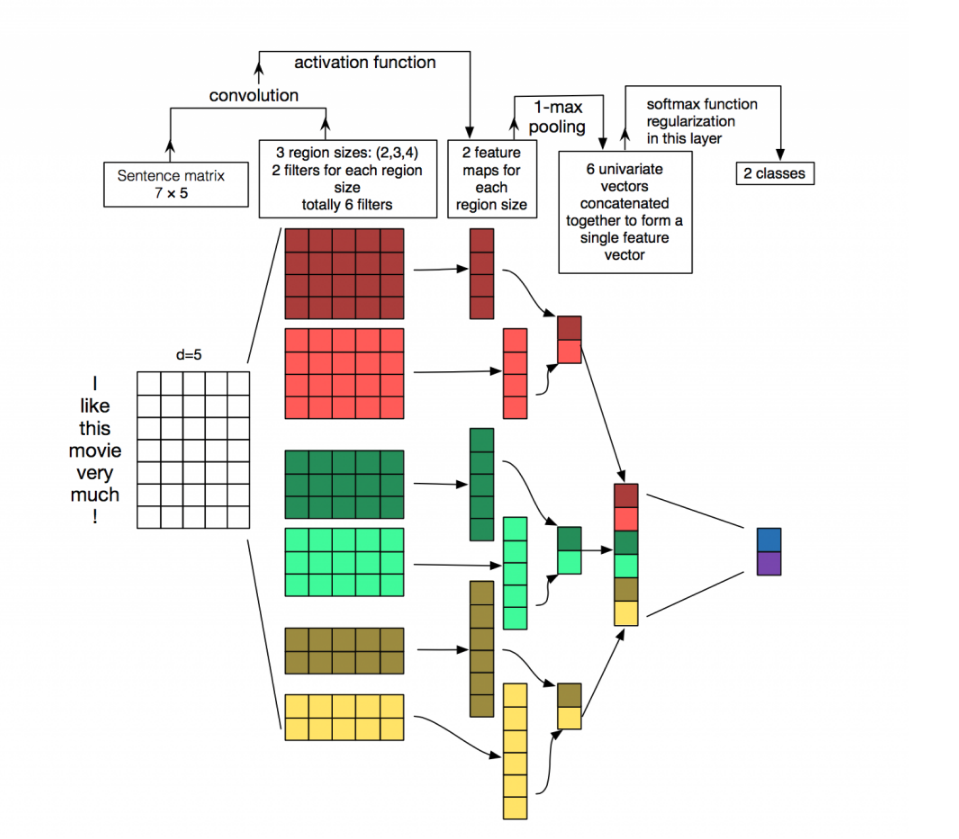
\includegraphics[width=0.5\textwidth]{images/cnn_architecture2.png}




The whole classification process can be sub-divided into two elementary parts
\begin{enumerate}
\item Feeding input data to Neural Network
\item Classifying data to correct class
\end{enumerate}
The following steps were taken in order to feed data to the Neural Network:
\begin{enumerate}
\item 7 raw text files were prepared each containing the tweets for respective parties collected from Twitter.
\item The dataset was cleaned and tokenized for building a vocabulary.
\item Each sentence was padded to a max length. We append special $<$PAD$>$ tokens to all other sentences to make them equal of 35 words. Padding sentences to the same length is useful because it allows us to efficiently batch our data since each example in a batch must be of the same length.
\item For feature extraction from twitter data we needed a pretrained word-embeddings to represent every word in vector form. We use [[cite here]] word-embeddings pretrained on [[]] million tweets and having a 200 dimension vector representation of each word.  
\item Finally we built a vocabulary based on our collected data and map each word to an integer between 0 and 109933 (the vocabulary size). Each sentence becomes a vector of integers.
\end{enumerate}

For classifying the user tweets to the correct political party, the following two steps were performed:
\begin{enumerate}
	\item We feed the batches of twitter data along with their correct political party one-hot-encoded labels and trained above defined CNN 
	\item To optimize the network we used the cross entropy loss defined as:
\end{enumerate}
\begin{equation}
%x =y+z
H_{y'}(y) = - \sum_{i} y'_{i} \log (y_{i})
\end{equation}
Where $y$ is our predicted probability distribution, and $y'$ is the true distribution (the one-hot vector with the true-class party labels). 


\section{Quantitative Analysis}

For quantitative analysis of the results, every tweets were taken as sentences and a sentence vector was constructed of the same dimension as the word vectors used for training (i.e. 200 dimensional vector). In doing so, the tweet was tokenized into words and every word corresponding token vectors were taken from the word embedding space and a sentence embedding vector was constructed by adding the word vectors and dividing them with the number of words. Only those tweets were considered whose all words were present in the word embedding space and any tweets with UNK token were ignored for better analysis. This was done to remove any tweets that were not completely related to politics as a user tweets on a variety of backgrounds and we only want the tweets related to political spectrum. 

The sentence embedding was used to visualize the vectors based on their 200-dimensional vector representations. The results were pretty mixed up with no clear distinct clusters for any specific party. There could be several reasons for the mixing up of results and no clear clusters. Since a user re-tweets other parties tweets with his opinions, it could be one of the reason for mixing up of clusters. 

Another reason for such mixed clusters is the fact every party is tweeting about the same issues with some in favor of it and some against of it and this leads to creation of same tokens for different party supporting user/group tweets. Further, these tweets with some/very less distinct tokens like together in the cluster prohibiting a distinct cluster for each class.

So a direct embedding as above did not proved to be a good measure to visualize the result. So we used a political compass for visualizing the result further. 

For the political compass representation, we use a four way graph plot with [[]] and [[]] on both the axis. On the four axis, we used an one hot encoding to plot all the seven classes on the compass. This way we can see all the political classes plotted. 

\subsection{Visualization}

Now, we need to plot all the users on the compass to see which users corresponds to what cluster and following steps were taken in order to do so:
\begin{enumerate}
	\item We take a user and scrape all the tweets of the user from twitter.
	\item Next we pass the tweets of the user to the classification model as specified above in the model architecture.
	\item We get the class classification and probability score  of all the tweets for all the seven classes.
	\item We average all the probability distribution to get one vector consisting of a probability distribution for all seven classes.
	\item We plot the user on the political compass to visualize the results and to see if the user has been classified to it’s correct class.
\end{enumerate}

\subsection{Inference}

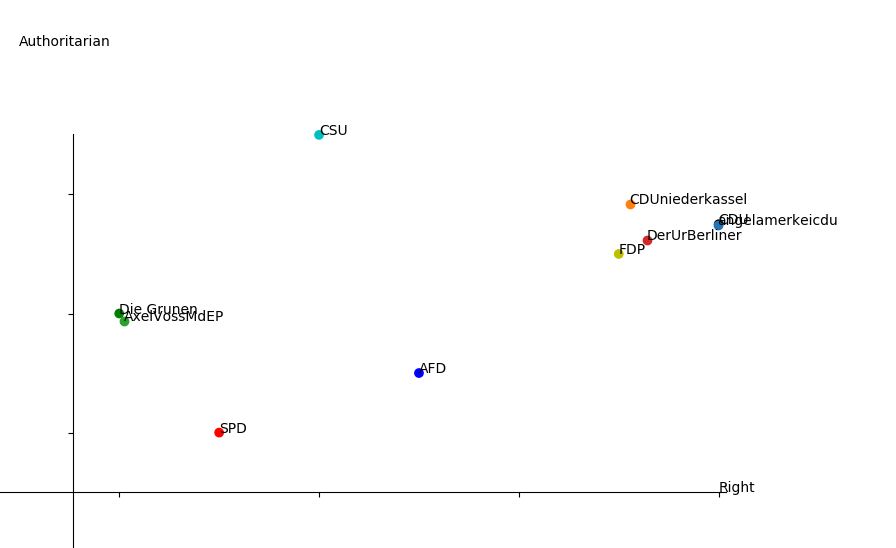
\includegraphics[width=0.5\textwidth]{images/Political_Compass.png}
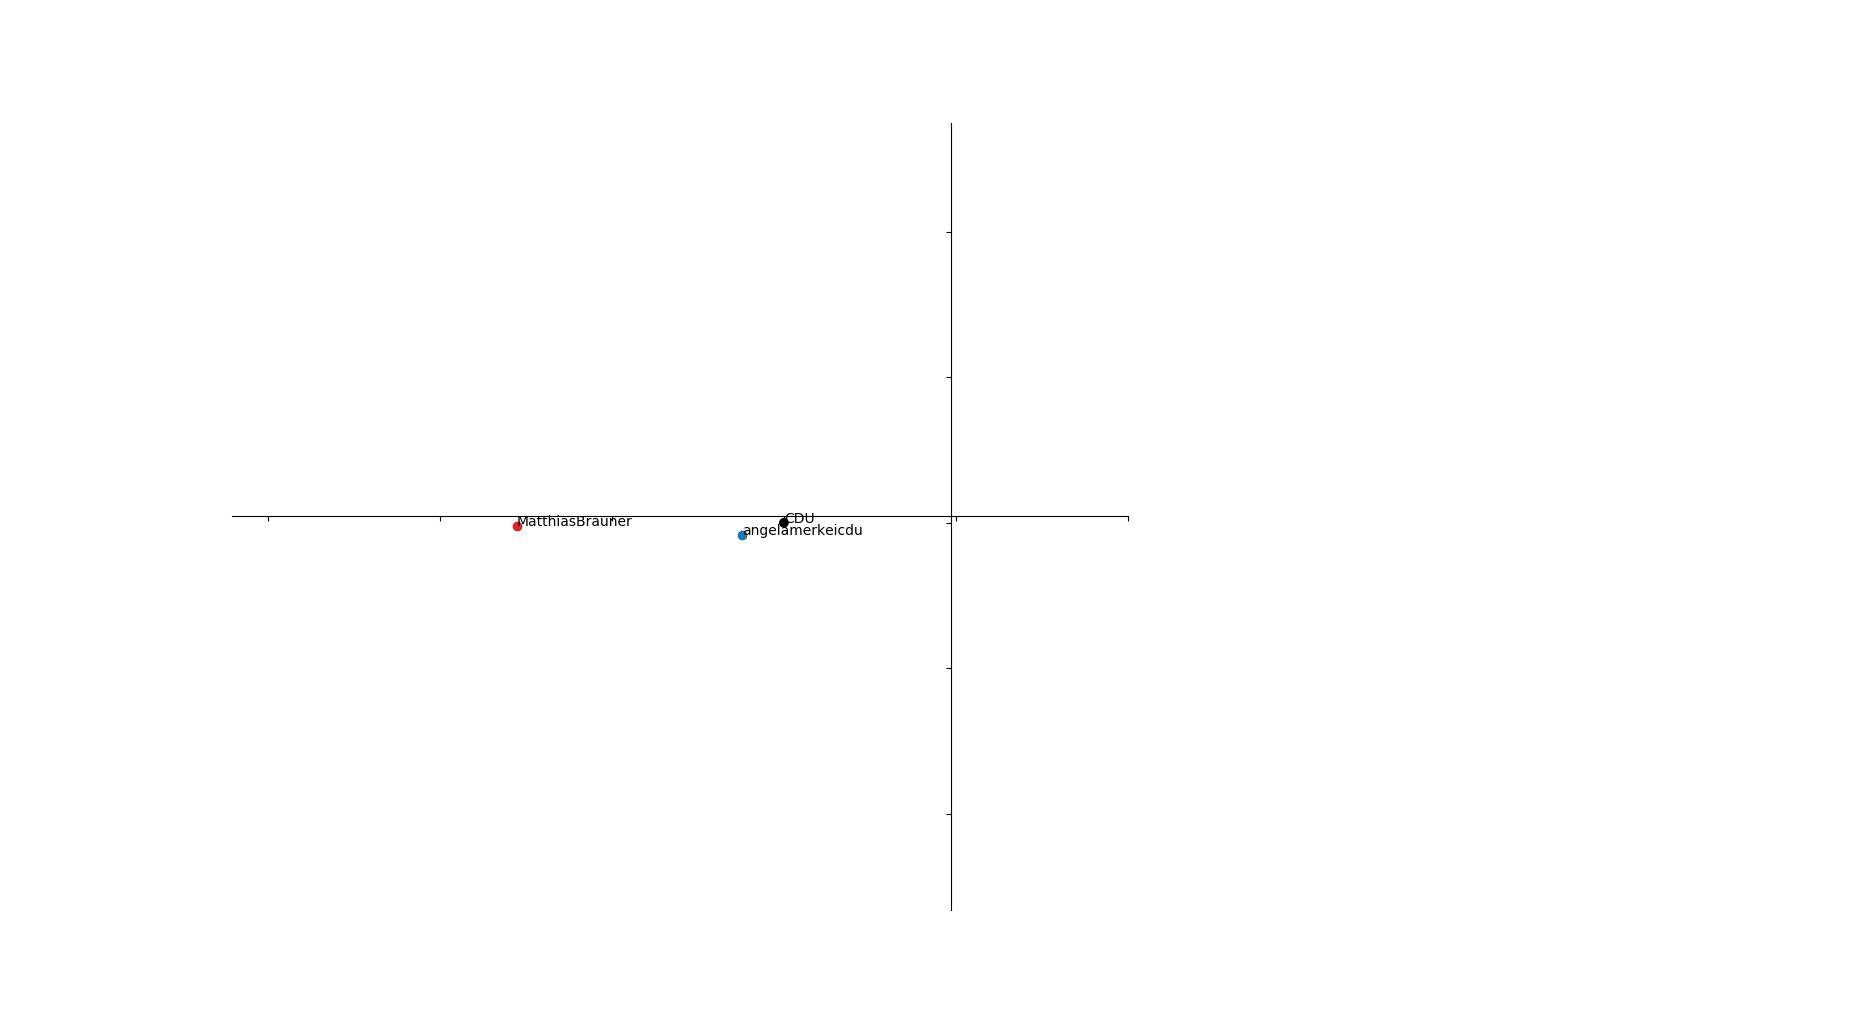
\includegraphics[width=0.5\textwidth]{images/Political_Compass-1.png}

The following can be inferred from the above political compass visualization:

\begin{enumerate}
	\item Most users have been plotted very near to it’s political party representation. E.q. Angela Merkel plot is very near to CDU which shows all her tweets were pretty biased for the CDU Party.
	\item Some plots like [[]] is very near to [[]] class. This means the ideology of these parties are quite similar. (Not exactly similar but some similarity is there.) This could also be seen from the usage of similar vocabulary used be both the parties.
	\item User [[]] from party [[]] is being classified to wrong party. [[]] in this case. Upon analyzing the data, it can be inferred that there are a lot of English language based tweets present in the scraped tweets which led to a lot of $<$UNK$>$ token generation and hence the classification was not correct. Upon data cleaning we were able to see the user plot moving to the correct class. 
\end{enumerate}


\end{multicols}
\newpage

\section{Appendix - Work packages and distribution}

We plan to distribute the workload into the work packages, for each work package we assign a group of people, and an initial estimated deadline.

\begin{flushleft}
\textbf{Building dataset}

Beside the Tweets of German politicians that we will get using the Twitter API, we also plan to collect data from other sources such as parliament discussion data and party manifesto data.
\end{flushleft}

\begin{flushleft}
\textbf{Training word vector model}

After building our dataset we will convert the data text into numerically creating word embedding of the words in the text using Word2Vec or derived approaches.
\end{flushleft}

\begin{flushleft}
\textbf{Developing classification model}

As previously mentioned in the Proposed Methodology we will implement a neural network as our classifier, and train it with our data set.
\end{flushleft}

\begin{flushleft}
\textbf{Training / Testing}

After having quantified model accuracy with a dedicated validation split, this separate training- and testing-stage ensures that the obtained results match initial expectations or reject estimates in an understandable fashion. We thereby ensure that the obtained results obey logic and real-world measures.
\end{flushleft}

\begin{flushleft}
\textbf{Quantitative Analysis}

To conclude the findings from real-word social media data analysis, we infer statistical and sociological meaning to the modeled results and put them in context to the initially motivated research question of political affiliation and political classification.
\end{flushleft}

\begin{sidewaysfigure}
  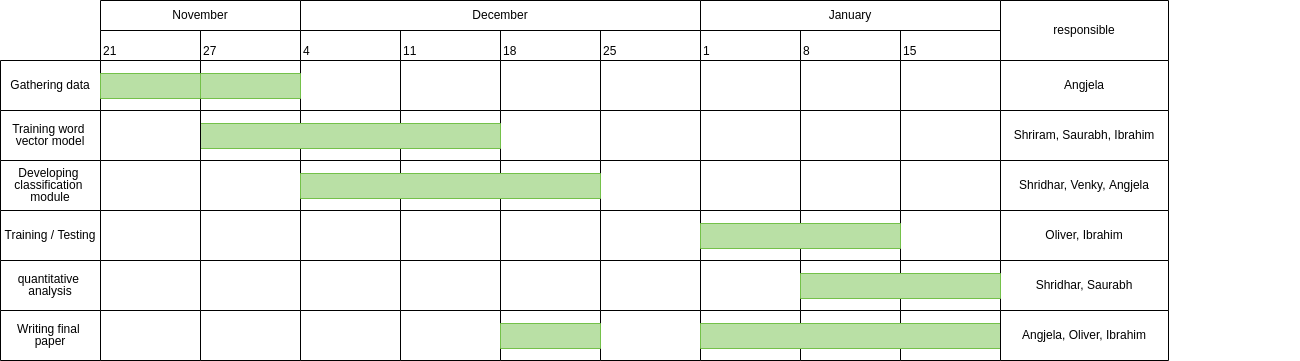
\includegraphics[width=\textwidth]{gantt.png}
  \caption{Gantt-Chart displaying workload distribution per team-member}
\end{sidewaysfigure}


\bibliography{lit}
\bibliographystyle{apalike}

\end{document} 
